\documentclass{article}

% preamble
\usepackage{tabularx}
\usepackage{booktabs}
\usepackage{xcolor}
\usepackage{colortbl}
\usepackage{array}
\usepackage{longtable}
\usepackage{graphicx}
\usepackage[left=0.25in, right=0.25in, top=0.5in, bottom=0.5in]{geometry}

% title
\title{Data methodology and observability}
\author{Charles T. Gray}

\begin{document}

\maketitle

\tableofcontents


\begin{abstract}
Validation and observability of prioritisation of UN SDGs represented in two surveys facilitated and collected by Garima Gupta. Participants in one survey from the North Indian regions Tehri and the other survey participants from Arunachal Pradesh. 

This document outlines the data methodology of the github repository and observability framework for data governance. 

This project employs a structured approach to data management, ensuring data quality, integrity, and usability through various layers of data observability. The observability framework is designed to monitor and validate data at each stage of the pipeline, providing transparency, accountability, and extensiblity in the data handling processes.

This document and the associated data are curated for submission to the beta rollout of the Frontiers FAIR data management platform.

\end{abstract}

\section{What are these data?}

The data in this project aggregates two region-based surveys, with responses from participants in Tehri and Arunachal Pradesh, focusing on their ranked top three priorities of the United Nations Sustainable Development Goals (UN SDGs). The data was collected by Garima Gupta by surveying residents of the two regions in Hindi. The data is stored in the \texttt{analysis\_data} directory. This project was created by Charles T. Gray  to aggregate survey responses across regions to investigate the following question.

\begin{quote}
  \textit{What are the differences in SDG priorities between residents of Tehri, where a dam was constructed 20 years ago for hydroelectric power, and Arunachal Pradesh, where a dam is currently being developed?}
\end{quote}

Figure \ref{fig:top3-treemap} shows a treemap of the top 3 UN SDG priorities from survey respondents in Tehri (dam constructed 20 years ago) and Arunachal Pradesh (dam under development), North India.

\begin{figure}[ht]
  \centering
  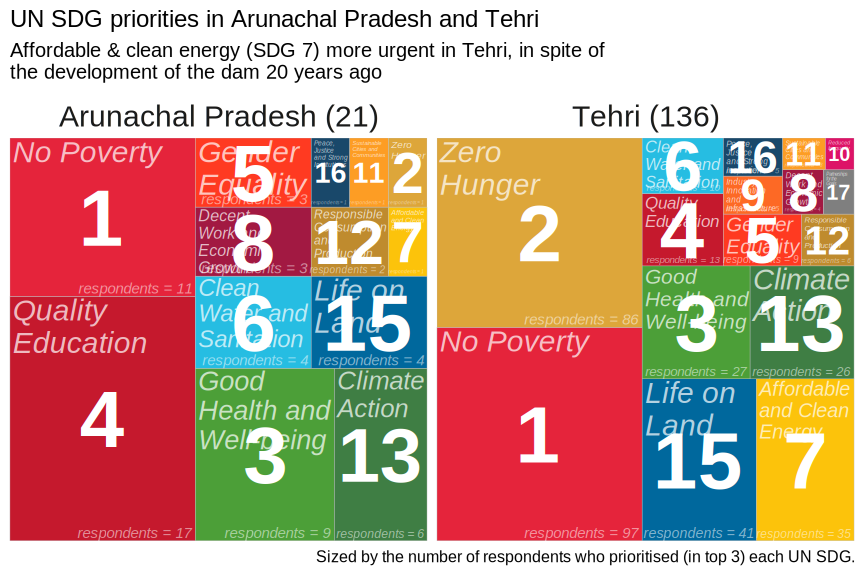
\includegraphics[width=0.95\textwidth]{../figures_and_tables/top3-treemap.png}
  \caption{\label{fig:top3-treemap} Treemap of top 3 UN SDG priorities from survey respondents in Tehri (dam constructed 20 years ago) and Arunachal Pradesh (dam under development), North India. Each rectangle represents a specific UN SDG, with its size proportional to the number of respondents who ranked it among their top three priorities. The treemap visually highlights the most and least prioritized SDGs in each region, providing insights into regional differences in development priorities.}
\end{figure}

By structuring the data in tidy format (one row per ranking by one respondent), 

\section{This data is FAIR}

\subsection{Findable}

CSV files respresenting respondent metadata and top 3 priorities of UN SDGs are found in \texttt{analysis\_data}. The data are described in the \texttt{data\_dictionary.md} file. The data are version controlled in the github repository \texttt{sig\_gg}.

\subsection{Accessible}

The data are provided in tidy format with descriptions, columns, and validations detailed in DBT. Column names were chosen for interpreability. 

\subsubsection{Responses to top 3 priorities of UN SDGs}

These responses are enriched with respondent metadata that corresponds to the respondent dataset also provided. 
\begin{itemize}
  \item \textbf{response\_id:} Unique identifier for each response.
  \item \textbf{respondent\_id:} Unique identifier for each respondent
  \item \textbf{region:} Region where the data was collected (Tehri or Arunachal Pradesh).
  \item \textbf{sdg\_rank:} Rank of the UN SDG priority (1, 2, or 3).
  \item \textbf{sdg\_number:} Unique identifier for each UN SDG (1-17).
  \item \textbf{sdg\_label:} UN SDG as text label.
  \item \textbf{age:} Age of the respondent.
  \item \textbf{gender:} Gender of the respondent.
  \item \textbf{displacement\_status:} Displacement status of the respondent.
\end{itemize}

By enriching the responses with respondent metadata, we can analyse responses in the context of respondent demographics and characteristics. For example, in Figure~\ref{fig:top3-gender-treemap}, we can see the distribution of top 3 UN SDG priorities by gender.

\begin{figure}[ht]
  \centering
  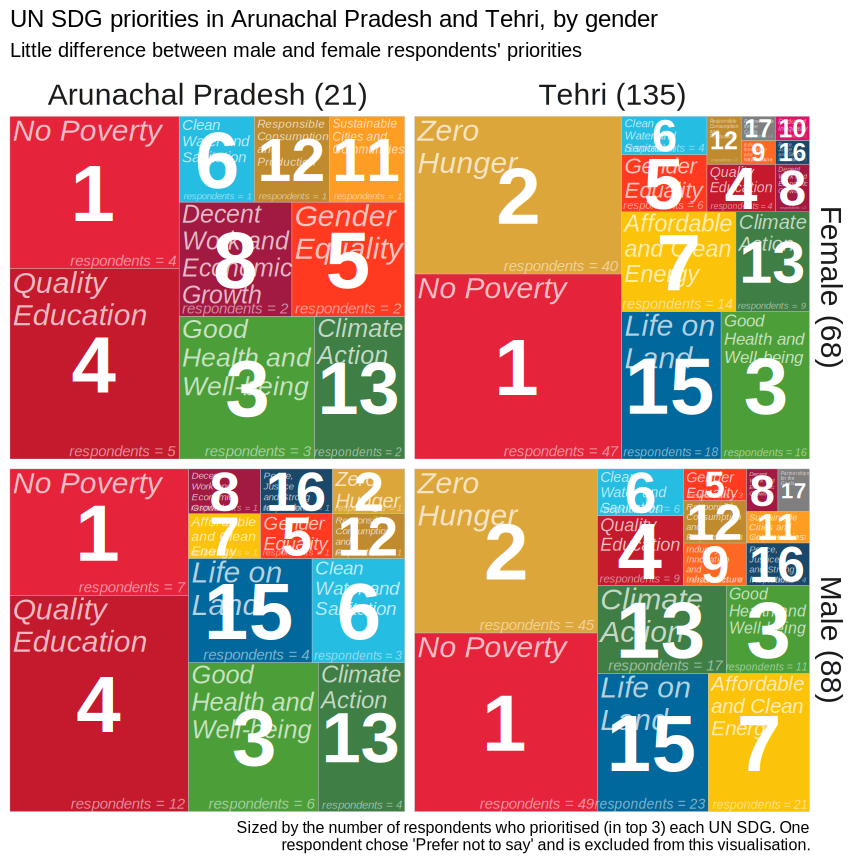
\includegraphics[width=0.95\textwidth]{../figures_and_tables/top3-gender-treemap.png}
  \caption{\label{fig:top3-gender-treemap} Treemap of top 3 UN SDG priorities from survey respondents in Tehri and Arunachal Pradesh, North India, by gender. Each rectangle represents a specific UN SDG, with its size proportional to the number of respondents of a particular gender who ranked it among their top three priorities. The treemap visually highlights the most and least prioritized SDGs in each region, providing insights into gender differences in development priorities.}
\end{figure}


\subsubsection{Respondent metadata}

\begin{itemize}
  \item \textbf{respondent\_id:} Unique identifier for each respondent.
  \item \textbf{region:} Region where the data was collected (Tehri or Arunachal Pradesh).
  \item \textbf{age:} Age of the respondent.
  \item \textbf{gender:} Gender of the respondent.
  \item \textbf{displacement\_status:} Displacement status of the respondent.
\end{itemize}

\subsection{Interoperable}

The data are published in \texttt{.csv} format on a publically available github repository \texttt{sig\_gg}, readable by url into Python or R.  

\subsection{Reusable}

The data pipeline is extensible. The repository can be forked and the DBT pipeline extended to transform the data in additional ways or patch in additional source data. The data are licensed under a Creative Commons Attribution 4.0 International (CC BY 4.0) license, allowing others to share and adapt the data with appropriate credit.

\section{Data lineage}

In \texttt{raw\_data} the original two survey data are found. To aggregate across the \texttt{.csv} and Kobo tool data export in \texttt{.xlsx} format, a data transformation pipeline was implemented using the Data Build Tool (DBT) in the \texttt{dbt\_project} directory. The DBT project consists of SQL scripts, tests, and documentation that transform the raw data into a tidy format suitable for analysis. Identifying which columns to extract from the Kobo export was nontrivial, \texttt{scripts/tehri-cols.R} contains the script used to identify the relevant columns, and a markdown table identifying the columns associated with survey questions can be found in \texttt{analysis\_data/tehri.md}.

Figure~\ref{fig:dbtdag} shows the directed acyclic graph (DAG) for the Data Build Tool (DBT) project \texttt{dbt\_project} that produced the .csv data found in \texttt{analysis\_data}. The DAG illustrates the relationships and dependencies between various data models, tests, and sources within the project. Each node represents a table produced during transformation, while the edges indicate the flow of data and dependencies among them. This visualization illustrates how data is transformed and validated throughout the pipeline, ensuring data integrity and reliability.

\begin{figure}[ht]
\centering
\includegraphics[width=\textwidth]{img/dbt-dag.png}
\caption{Data Build Tool (DBT) directed acyclic graph (DAG).}
\label{fig:dbtdag}
\end{figure}

Table~\ref{tab:dbt_models} lists the DBT models created by the \texttt{dbt\_project}, ordered by observability layer. 

\begin{table}[!h]
\centering
\caption{\label{tab:dbt_models}Data Build Tool (DBT) models created by dbt\_project, ordered by observability layer.}
\centering
\fontsize{8}{10}\selectfont
\begin{tabular}[t]{>{\raggedright\arraybackslash}p{0.18\textwidth}>{\raggedright\arraybackslash}p{0.75\textwidth}}
\toprule
Model & Description\\
\midrule
\addlinespace[0.3em]
\multicolumn{2}{l}{\textbf{Analytic Models}}\\
\hspace{1em}\cellcolor{gray!10}{ana\_respondents} & \cellcolor{gray!10}{NA}\\
\hspace{1em}ana\_top3 & NA\\
\addlinespace[0.3em]
\multicolumn{2}{l}{\textbf{Semantic Models}}\\
\hspace{1em}\cellcolor{gray!10}{sem\_respondents} & \cellcolor{gray!10}{NA}\\
\hspace{1em}sem\_sdg\_labels & NA\\
\hspace{1em}\cellcolor{gray!10}{sem\_top3} & \cellcolor{gray!10}{NA}\\
\addlinespace[0.3em]
\multicolumn{2}{l}{\textbf{Source Entity Models}}\\
\hspace{1em}se\_respondents\_arunachal & Each row represents a respondent from Arunachal Pradesh.\\
\hspace{1em}\cellcolor{gray!10}{se\_respondents\_tehri} & \cellcolor{gray!10}{Each row represents a respondent from Tehri.}\\
\hspace{1em}se\_top3\_arunachal & Each row represents a respondent's ranking of their top 3 UN Sustainable Development Goals (SDGs) for Arunachal Pradesh, India.\\
\hspace{1em}\cellcolor{gray!10}{se\_top3\_tehri} & \cellcolor{gray!10}{Each row represents a respondent's ranking of their top 3 UN Sustainable Development Goals (SDGs) for Tehri, India.}\\
\addlinespace[0.3em]
\multicolumn{2}{l}{\textbf{Base Models}}\\
\hspace{1em}base\_arunachal & Raw data from survey in Arunachal Pradesh, collected by Dr Garima Gupta. Each row represents the survey responses of a single respondent.\\
\hspace{1em}\cellcolor{gray!10}{base\_tehri} & \cellcolor{gray!10}{Raw data from survey in Tehri, collected by Dr Garima Gupta. Each row represents the survey responses of a single respondent.}\\
\bottomrule
\end{tabular}
\end{table}


\section{Data observability}

\subsection{Layers}

The data observability framework implemented in the \texttt{dbt\_project} is structured into four distinct layers: base models, source entities, semantic models, and analytic models. Each layer serves a specific purpose in ensuring data quality, integrity, and usability throughout the data pipeline.

\begin{itemize}
    \item \textbf{Base Models:} These are the foundational models that directly interact with raw data sources. They perform initial data extraction and loading (ETL) processes to prepare the data for further analysis. Base models focus on cleaning and structuring the data to ensure it is in a usable format. These models were loaded from CSV files as seeds. The script to convert the raw files to csv to be seeded is found in \texttt{scripts/seed-data.R}.

    \item \textbf{Source Entities:} This layer represents the core data entities (responses and respondents) by source derived from the base models for respondents and responses. This layer allows for easier validation of data integrity as each source has different labelling and structure.
    
    \item \textbf{Semantic Models:} Semantic models aggregate source entities to semantic entities: respondents, responses. This layer ensures the consistency of labelling, for example, UN SDGs were labelled very differently in the two datasets.
    
    \item \textbf{Analytic Models:} The analytic layer enriched semantic data. For example, responses are enriched with respondent metadata such as region, age, gender, and displacement status. 
\end{itemize}

\subsection{Data validation}

Table~\ref{tab:dbt_tests} lists the DBT tests applied to \texttt{dbt\_project} transformations, ordered by observability layer. These tests tell us what assumptions we have validated at each transformation step in the lineage (Figure~\ref{fig:dbtdag}).

\begin{table}[!h]
\centering
\caption{\label{tab:dbt_tests}Data Build Tool (DBT) tests applied to dbt\_project models, ordered by observability layer.}
\centering
\fontsize{8}{10}\selectfont
\begin{tabular}[t]{>{\raggedright\arraybackslash}p{0.20\textwidth}>{\raggedright\arraybackslash}p{0.20\textwidth}>{\raggedright\arraybackslash}p{0.10\textwidth}>{\raggedright\arraybackslash}p{0.25\textwidth}>{\raggedright\arraybackslash}p{0.10\textwidth}}
\toprule
Model & Test & Columns & Arguments & Result\\
\midrule
\addlinespace[0.3em]
\multicolumn{5}{l}{\textbf{Analytic Model Tests}}\\
\hspace{1em}\hspace{1em}\cellcolor{gray!10}{ana\_respondents} & \cellcolor{gray!10}{unique\_combination\_of\_columns} & \cellcolor{gray!10}{id\_respondent} & \cellcolor{gray!10}{NA} & \cellcolor{gray!10}{pass}\\
\addlinespace[0.3em]
\multicolumn{5}{l}{\textbf{Semantic Model Tests}}\\
\addlinespace[0.3em]
\multicolumn{5}{l}{\textbf{Source Entity Tests}}\\
\hspace{1em}\hspace{1em}se\_respondents\_arunachal & accepted\_values & gender & Male\_\_Female\_\_Prefer\_not\_to\_say & pass\\
\hspace{1em}\cellcolor{gray!10}{se\_respondents\_arunachal} & \cellcolor{gray!10}{not\_null} & \cellcolor{gray!10}{id\_respondent} & \cellcolor{gray!10}{NA} & \cellcolor{gray!10}{pass}\\
\hspace{1em}se\_respondents\_arunachal & unique & id\_respondent & NA & pass\\
\hspace{1em}\cellcolor{gray!10}{se\_respondents\_arunachal} & \cellcolor{gray!10}{unique\_combination\_of\_columns} & \cellcolor{gray!10}{id\_respondent} & \cellcolor{gray!10}{NA} & \cellcolor{gray!10}{pass}\\
\hspace{1em}se\_respondents\_tehri & accepted\_values & gender & Male\_\_Female\_\_Prefer\_not\_to\_say & pass\\
\hspace{1em}\cellcolor{gray!10}{se\_respondents\_tehri} & \cellcolor{gray!10}{not\_null} & \cellcolor{gray!10}{id\_respondent} & \cellcolor{gray!10}{NA} & \cellcolor{gray!10}{pass}\\
\hspace{1em}se\_respondents\_tehri & unique & id\_respondent & NA & pass\\
\hspace{1em}\cellcolor{gray!10}{se\_respondents\_tehri} & \cellcolor{gray!10}{unique\_combination\_of\_columns} & \cellcolor{gray!10}{id\_respondent} & \cellcolor{gray!10}{NA} & \cellcolor{gray!10}{pass}\\
\hspace{1em}se\_top3\_arunachal & accepted\_values & rank & 1\_\_2\_\_3 & pass\\
\hspace{1em}\cellcolor{gray!10}{se\_top3\_arunachal} & \cellcolor{gray!10}{not\_null} & \cellcolor{gray!10}{id\_respondent} & \cellcolor{gray!10}{NA} & \cellcolor{gray!10}{pass}\\
\hspace{1em}se\_top3\_arunachal & unique\_combination\_of\_columns & id\_respondent & rank & pass\\
\hspace{1em}\cellcolor{gray!10}{se\_top3\_tehri} & \cellcolor{gray!10}{accepted\_values} & \cellcolor{gray!10}{rank} & \cellcolor{gray!10}{1\_\_2\_\_3} & \cellcolor{gray!10}{pass}\\
\hspace{1em}se\_top3\_tehri & not\_null & id\_respondent & NA & pass\\
\hspace{1em}\cellcolor{gray!10}{se\_top3\_tehri} & \cellcolor{gray!10}{unique\_combination\_of\_columns} & \cellcolor{gray!10}{id\_respondent} & \cellcolor{gray!10}{rank} & \cellcolor{gray!10}{pass}\\
\addlinespace[0.3em]
\multicolumn{5}{l}{\textbf{Base Model Tests}}\\
\hspace{1em}base\_arunachal & unique\_combination\_of\_columns & id\_respondent & NA & pass\\
\hspace{1em}\cellcolor{gray!10}{base\_arunachal} & \cellcolor{gray!10}{unique\_combination\_of\_columns} & \cellcolor{gray!10}{respondents} & \cellcolor{gray!10}{NA} & \cellcolor{gray!10}{pass}\\
\hspace{1em}base\_tehri & not\_null & id\_respondent & NA & pass\\
\hspace{1em}\cellcolor{gray!10}{base\_tehri} & \cellcolor{gray!10}{unique} & \cellcolor{gray!10}{id\_respondent} & \cellcolor{gray!10}{NA} & \cellcolor{gray!10}{pass}\\
\hspace{1em}base\_tehri & unique\_combination\_of\_columns & id & NA & pass\\
\hspace{1em}\cellcolor{gray!10}{base\_tehri} & \cellcolor{gray!10}{unique\_combination\_of\_columns} & \cellcolor{gray!10}{id\_respondent} & \cellcolor{gray!10}{NA} & \cellcolor{gray!10}{pass}\\
\bottomrule
\end{tabular}
\end{table}



\end{document}